%%%%%%%%%%%%%%%%%%%%%%%%%%%%%%%%%%%%%%%%%
% Beamer Presentation
% LaTeX Template
% Version 1.0 (10/11/12)
%
% This template has been downloaded from:
% http://www.LaTeXTemplates.com
%
% License:
% CC BY-NC-SA 3.0 (http://creativecommons.org/licenses/by-nc-sa/3.0/)
%
%%%%%%%%%%%%%%%%%%%%%%%%%%%%%%%%%%%%%%%%%

%----------------------------------------------------------------------------------------
%	PACKAGES AND THEMES
%----------------------------------------------------------------------------------------

\documentclass{beamer}

\mode<presentation> {

% The Beamer class comes with a number of default slide themes
% which change the colors and layouts of slides. Below this is a list
% of all the themes, uncomment each in turn to see what they look like.

%\usetheme{default}
%\usetheme{AnnArbor}
%\usetheme{Antibes}
%\usetheme{Bergen}
%\usetheme{Berkeley}
%\usetheme{Berlin}
%\usetheme{Boadilla}
%\usetheme{CambridgeUS}
%\usetheme{Copenhagen}
%\usetheme{Darmstadt}
%\usetheme{Dresden}
\usetheme{Frankfurt}
%\usetheme{Goettingen}
%\usetheme{Hannover}
%\usetheme{Ilmenau}
%\usetheme{JuanLesPins}
%\usetheme{Luebeck}
%\usetheme{Madrid}
%\usetheme{Malmoe}
%\usetheme{Marburg}
%\usetheme{Montpellier}
%\usetheme{PaloAlto}
%\usetheme{Pittsburgh}
%\usetheme{Rochester}
%\usetheme{Singapore}
%\usetheme{Szeged}
%\usetheme{Warsaw}

% As well as themes, the Beamer class has a number of color themes
% for any slide theme. Uncomment each of these in turn to see how it
% changes the colors of your current slide theme.

%\usecolortheme{albatross}
%\usecolortheme{beaver}
%\usecolortheme{beetle}
%\usecolortheme{crane}
%\usecolortheme{dolphin}
%\usecolortheme{dove}
%\usecolortheme{fly}
%\usecolortheme{lily}
%\usecolortheme{orchid}
%\usecolortheme{rose}
%\usecolortheme{seagull}
%\usecolortheme{seahorse}
%\usecolortheme{whale}
%\usecolortheme{wolverine}

%\setbeamertemplate{footline} % To remove the footer line in all slides uncomment this line
%\setbeamertemplate{footline}[page number] % To replace the footer line in all slides with a simple slide count uncomment this line

%\setbeamertemplate{navigation symbols}{} % To remove the navigation symbols from the bottom of all slides uncomment this line
}
\usepackage{graphicx} % Allows including images
\usepackage{subimages}
\usepackage{media9}
\usepackage{booktabs} % Allows the use of \toprule, \midrule and \bottomrule in tables
\usepackage[brazilian]{babel}
\usepackage[utf8]{inputenc}
\usepackage[T1]{fontenc}
\usepackage{amsmath}
\usepackage{animate}
\usepackage{amsmath}
\DeclareMathOperator{\atantwo}{atan2}
\newcommand{\angstrom}{\textup{\AA}}

%----------------------------------------------------------------------------------------
%	TITLE PAGE
%----------------------------------------------------------------------------------------

\title[T2]{Visualização de simulações de dinâmica molecular} % The short title appears at the bottom of every slide, the full title is only on the title page

\author{Bruno Iochins Grisci} % Your name
\institute[UFRGS] % Your institution as it will appear on the bottom of every slide, may be shorthand to save space
{
Universidade Federal do Rio Grande do Sul \\ % Your institution for the title page
\medskip
\textit{bigrisci@inf.ufrgs.br} % Your email address
}
\date{\today} % Date, can be changed to a custom date

\begin{document}

\begin{frame}
\titlepage % Print the title page as the first slide
\end{frame}

\begin{frame}
\frametitle{Sumário} % Table of contents slide, comment this block out to remove it
\tableofcontents % Throughout your presentation, if you choose to use \section{} and \subsection{} commands, these will automatically be printed on this slide as an overview of your presentation
\end{frame}

%----------------------------------------------------------------------------------------
%	PRESENTATION SLIDES
%----------------------------------------------------------------------------------------

%------------------------------------------------
\section{Introdução} % Sections can be created in order to organize your presentation into discrete blocks, all sections and subsections are automatically printed in the table of contents as an overview of the talk
%------------------------------------------------

\begin{frame}
\frametitle{Proteínas}
\begin{itemize}
\item Proteínas são macromoléculas essenciais para o funcionamento do organismo dos seres-vivos.
\item São formadas por uma sequência unidimensional de amino ́ácidos própria e única.
\item Na natureza, existem 20 cadeias laterais, diferenciando os 20 amino ́ácidos básicos.
\end{itemize}
\begin{figure}
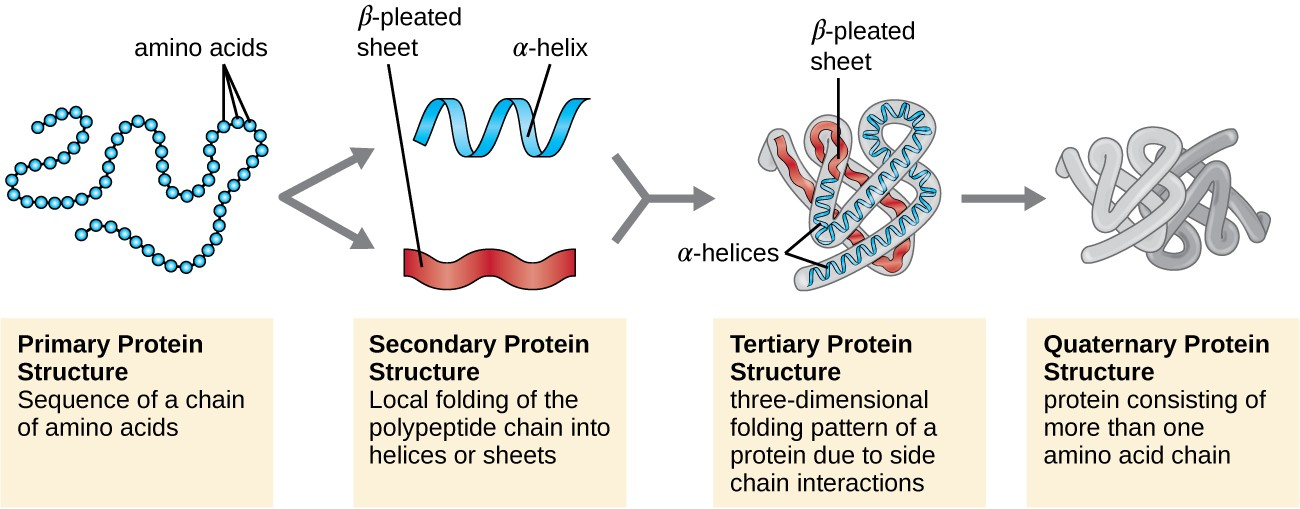
\includegraphics[width=0.7\linewidth]{figs/protein.jpg}
\caption{Estrutura das proteínas.} 
\label{fig:protein}
\end{figure}
\end{frame}

\begin{frame}
\frametitle{Dinâmica Molecular}
\begin{figure}
    \centering
    \includemedia[
    width=0.6\linewidth,height=0.3375\linewidth,
    activate=pageopen,
    flashvars={
        modestbranding=1 % no YT logo in control bar
        &autohide=1 % controlbar autohide
        &showinfo=0 % no title and other info before start
        &rel=0 % no related videos after end
    }
        ]{}{https://www.youtube.com/watch?v=Aj5f0XSv0t8}
\end{figure}
\end{frame}

\begin{frame}
\frametitle{Dimensões}
\begin{itemize}
\item DSSP: estrutura secundária
\item SASA: solvent-accessible surface area
\item GYRATE: raio de giro
\item ENERGY: energia total do sistema
\item RMSF: root mean square fluctuation of atomic positions
\end{itemize}
Todas as dimensões são valores numéricos contínuos.
\end{frame}

\begin{frame}
\frametitle{Kappa-conotoxin PVIIA}
\begin{figure}
\includegraphics[width=0.9\linewidth]{figs/lesma.jpg}
\caption{Lesma marinha.} 
\label{fig:lesma}
\end{figure}
\end{frame}

\begin{frame}
\frametitle{Kappa-conotoxin PVIIA}
\begin{itemize}
 \item Toxina encontrada em lesmas marinhas.
 \item $CRIPNQKCFQHLDDCCSRKCNRFNKCV$
 \item Mutação da asparagina (N) na quinta posição por uma alanina (A) causa perda de 100\% da toxicidade.
\end{itemize}
\begin{figure}
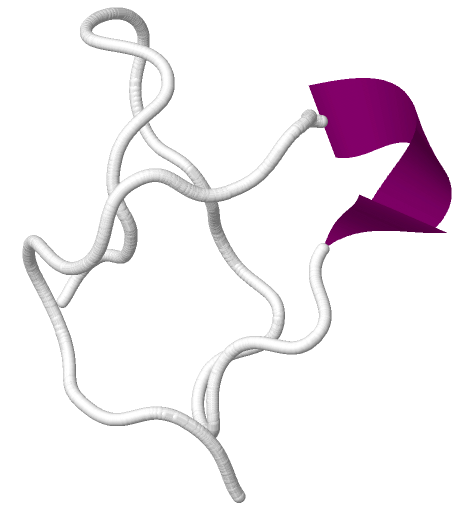
\includegraphics[width=0.3\linewidth]{figs/pviia.png}
\caption{Estrutura 3D da Kappa-conotoxin PVIIA.} 
\label{fig:pviia}
\end{figure}
\end{frame}

%------------------------------------------------
\section{Implementação} % Sections can be created in order to organize your presentation into discrete blocks, all sections and subsections are automatically printed in the table of contents as an overview of the talk
%------------------------------------------------

\begin{frame}
\frametitle{Ferramentas}
\begin{itemize}
\item JavaScript;
\item HTML;
\item CSS;
\item D3.js.
\end{itemize}
\end{frame}

%------------------------------------------------
\section{Ferramenta} % Sections can be created in order to organize your presentation into discrete blocks, all sections and subsections are automatically printed in the table of contents as an overview of the talk
%------------------------------------------------

\begin{frame}
\frametitle{Funcionalidades}
\begin{itemize}
\item Grid
  \begin{itemize}
  \item Destaque de item
  \item Seleção de item
  \end{itemize}
\item Parallel Coordinates
  \begin{itemize}
  \item Filtragem de eixo
  \item Ordenação de eixo
  \item Reposicionamento de eixo
  \item Coloração por seleção de eixo
  \end{itemize}
\item Radar Chart
  \begin{itemize}
  \item Destaque de item
  \end{itemize}
\item Slider
\end{itemize}
\end{frame}

%------------------------------------------------
\section{Resultados} % Sections can be created in order to organize your presentation into discrete blocks, all sections and subsections are automatically printed in the table of contents as an overview of the talk
%------------------------------------------------

\begin{frame}
\frametitle{Visão geral}
\begin{figure}
\includegraphics[width=0.8\linewidth]{figs/all.png}
\end{figure}
Disponível em: \url{http://inf.ufrgs.br/~bigrisci/parallel-coordinates}
\end{frame}

\begin{frame}
\frametitle{Comparação N x A}

\subimages[htb]{Comparação entre simulações com asparagina (amarelo) e alanina (vermelho) em 3 momentos distintos.}{fig:alaasn}{%
  \subimage[Time step 30000]{.3}{alaasn30000.png}%
  \subimage[Time step 40000]{.3}{alaasn40000.png}% 
  \subimage[Time step 50000]{.3}{alaasn50000.png}%
}
\end{frame}

\begin{frame}
\frametitle{Trabalhos futuros}
\begin{itemize}
\item Teste com outras proteínas;
\item Ferramenta web;
\item Adicionar novas visualizações;
\item Experimentar com outros tipos de dados.
\end{itemize}
\end{frame}

\begin{frame}
\Huge{\centerline{Obrigado :)}}
\end{frame}

%----------------------------------------------------------------------------------------

\end{document} 